\phantomsection\subsection*{Supplementary Note 4: NF2 positive-control benchmark}
\label{supp:enrichment-benchmark}

To compare enrichment methods on experimental DEL data with known binders,
we benchmarked six ranking methods on the NF2 DEL library
selections reported by Favalli et al.\cite{ref38}. The scores are defined in
Supplementary Note~3. All methods were applied to the same selection data and
evaluated against the same curated set of affinity-measured positive controls.


\textbf{Positive-control curation.}
Positive controls were defined by directly measured binding affinities (SPR
\kd{} or competitive ELISA IC$_{50}$) ranging from 7~nM to 6~$\mu$M. The
headline benchmark includes only compounds for which binding was confirmed by
resynthesis and measurement of an isolated disynthon, giving 14 target/display
instances across seven compound--target entries
(Supplementary Table~\ref{tab:strict_truth}).
Here, $n = 14$ means 14 positive-control instances across specific target and
display-condition pairs, not 14 unique chemical structures. Expanded curation
categories, including enrichment-only, weak-affinity, secondary cross-reactivity,
and negative or borderline rows, are retained in
\path{supporting_material/experiments/favalli/benchmark_nf2/truth_set.csv} but
are not included in headline recall.

\begin{table}[htbp]
\centering
\caption{\textbf{Strict-affinity positive controls used for the NF2-DEL enrichment benchmark.}
Conditions indicate whether the compound was evaluated in single-stranded (ss),
double-stranded (ds), or both display formats. Cpd refers to paper published numbered compounds.}
\label{tab:strict_truth}
\small
\ra{1.12}
\begin{tabular}{L{2.5cm} L{2.2cm} L{4.7cm} C{1.8cm} R{1.4cm}}
\toprule
Target & A/B pair & Evidence & Conditions & Instances \\
\midrule
CAIX & A160/B475 & Cpd 8/10, \kd{} 7.2--8.8 nM & ss, ds & 2 \\
CAIX & A69/B475  & Cpd 12, \kd{} 68 nM & ss, ds & 2 \\
CREBBP & A130/B99 & Cpd 13, \kd{} 0.92 \textmu{}M & ss, ds & 2 \\
CREBBP & A130/B128 & Cpd 14, \kd{} 6.0 \textmu{}M & ss, ds & 2 \\
wt-PI3K & A110/B489 & Cpd 16/17, \kd{} 306/126 nM & ss, ds & 2 \\
H1047R-PI3K & A110/B319 & Cpd 22/23, ELISA 0.19/0.37 \textmu{}M & ss, ds & 2 \\
H1047R-PI3K & A110/B157 & Cpd 20/21, ELISA 3.6/3.0 \textmu{}M & ss, ds & 2 \\
\midrule
\multicolumn{4}{r}{Total strict-affinity instances} & 14 \\
\bottomrule
\end{tabular}
\end{table}

\textbf{Control design.}
The benchmark uses the Favalli NF-DEL protein selections with strand-matched
no-protein controls. It covers 14 target/display-condition instances across
four protein targets: CAIX, CREBBP, wild-type PI3K, and H1047R-PI3K. The
published target selections were generated in triplicate for these conditions.
One CAIX ss count table (\texttt{NF2\_NatChem\_fl1\_1}) is excluded before rank
calculation on read-depth grounds: it contains only 488 total reads, compared
with 335,000--564,000 reads for the remaining CAIX ss tables, indicating an
incomplete or failed sequencing import rather than ordinary replicate noise.
The processed benchmark therefore uses two protein replicates for CAIX ss and
three protein replicates for the other seven conditions, paired with triplicate
strand-matched no-protein controls throughout. Across the eight ranked
conditions, each contains approximately 276,000--299,000 distinct observed
disynthons from a theoretical 334,764-member A/B count matrix (612 A-codes
$\times$ 547 B-codes). No-protein ss selections were used for ss comparisons,
and no-protein ds selections were used for ds comparisons.

\textbf{Benchmark metrics.}
All methods are evaluated on median rank, Recall@$k$, and worst rank. Median
rank captures the typical retrieval position of the known binder in its full
ranked output. Recall@$k$ reports the fraction of strict positives recovered
within the top $k$ positions, with Recall@10 representing a short inspection
list and Recall@50 a practical follow-up scale. Worst rank exposes individual
failures that would be masked by the median, particularly under low-read-depth
or near-detection-limit conditions.

\textbf{Summary results.}
Supplementary Table~\ref{tab:strict_summary_6method} summarizes performance across all six
methods on the 14 strict-affinity instances. \delthit{} counts,
\delthit{} z-score, and \deli{} NSC recover the known positives most
consistently, each reaching Recall@50 of 92.9\% (13/14) with median ranks of
1.5--2.0. \deli{} MLE and \delthit{} edgeR recover fewer positives
within the top 50, while \deli{} norm-z performs poorly in this sparse
no-protein-control setting. The assumptions behind these results are described
in Supplementary Note~3.

\begin{table}[htbp]
\centering
\caption{\textbf{Summary of positive-control recovery for all six methods
($n = 14$ strict-affinity instances).}
R@$k$ = Recall@$k$ (fraction of positives in the top-$k$ ranked compounds).
Bold = best per column. Lower median/worst rank and higher R@$k$ are better.}
\label{tab:strict_summary_6method}
\small
\ra{1.18}
\begin{tabular}{L{3.5cm} R{1.0cm} R{1.8cm} R{1.8cm} R{1.4cm} R{1.4cm} R{1.6cm}}
\toprule
Method & $n$ & Median rank & Worst rank & R@10 & R@50 & R@100 \\
\midrule
\delthit{} counts     & 14 & \textbf{1.5} & 31,730          & \textbf{0.857} & \textbf{0.929} & \textbf{0.929} \\
\delthit{} z-score & 14 & \textbf{2.0} & 674             & \textbf{0.857} & \textbf{0.929} & \textbf{0.929} \\
\deli{} NSC           & 14 & \textbf{2.0} & \textbf{425}    & \textbf{0.857} & \textbf{0.929} & \textbf{0.929} \\
\midrule
\deli{} MLE           & 14 & 30.5  & 161,254 & 0.357 & 0.571 & 0.571 \\
\delthit{} edgeR      & 14 & 46.0  & 136,360 & 0.286 & 0.500 & 0.571 \\
\deli{} norm-z        & 14 & 113,009 & 164,061 & 0.143 & 0.143 & 0.143 \\
\bottomrule
\end{tabular}
\end{table}

Supplementary Figure~\ref{fig:delt_vs_deli_recall} compares Recall@10, @50, and @100 grouped by tool family.

\begin{figure}[htbp]
\centering
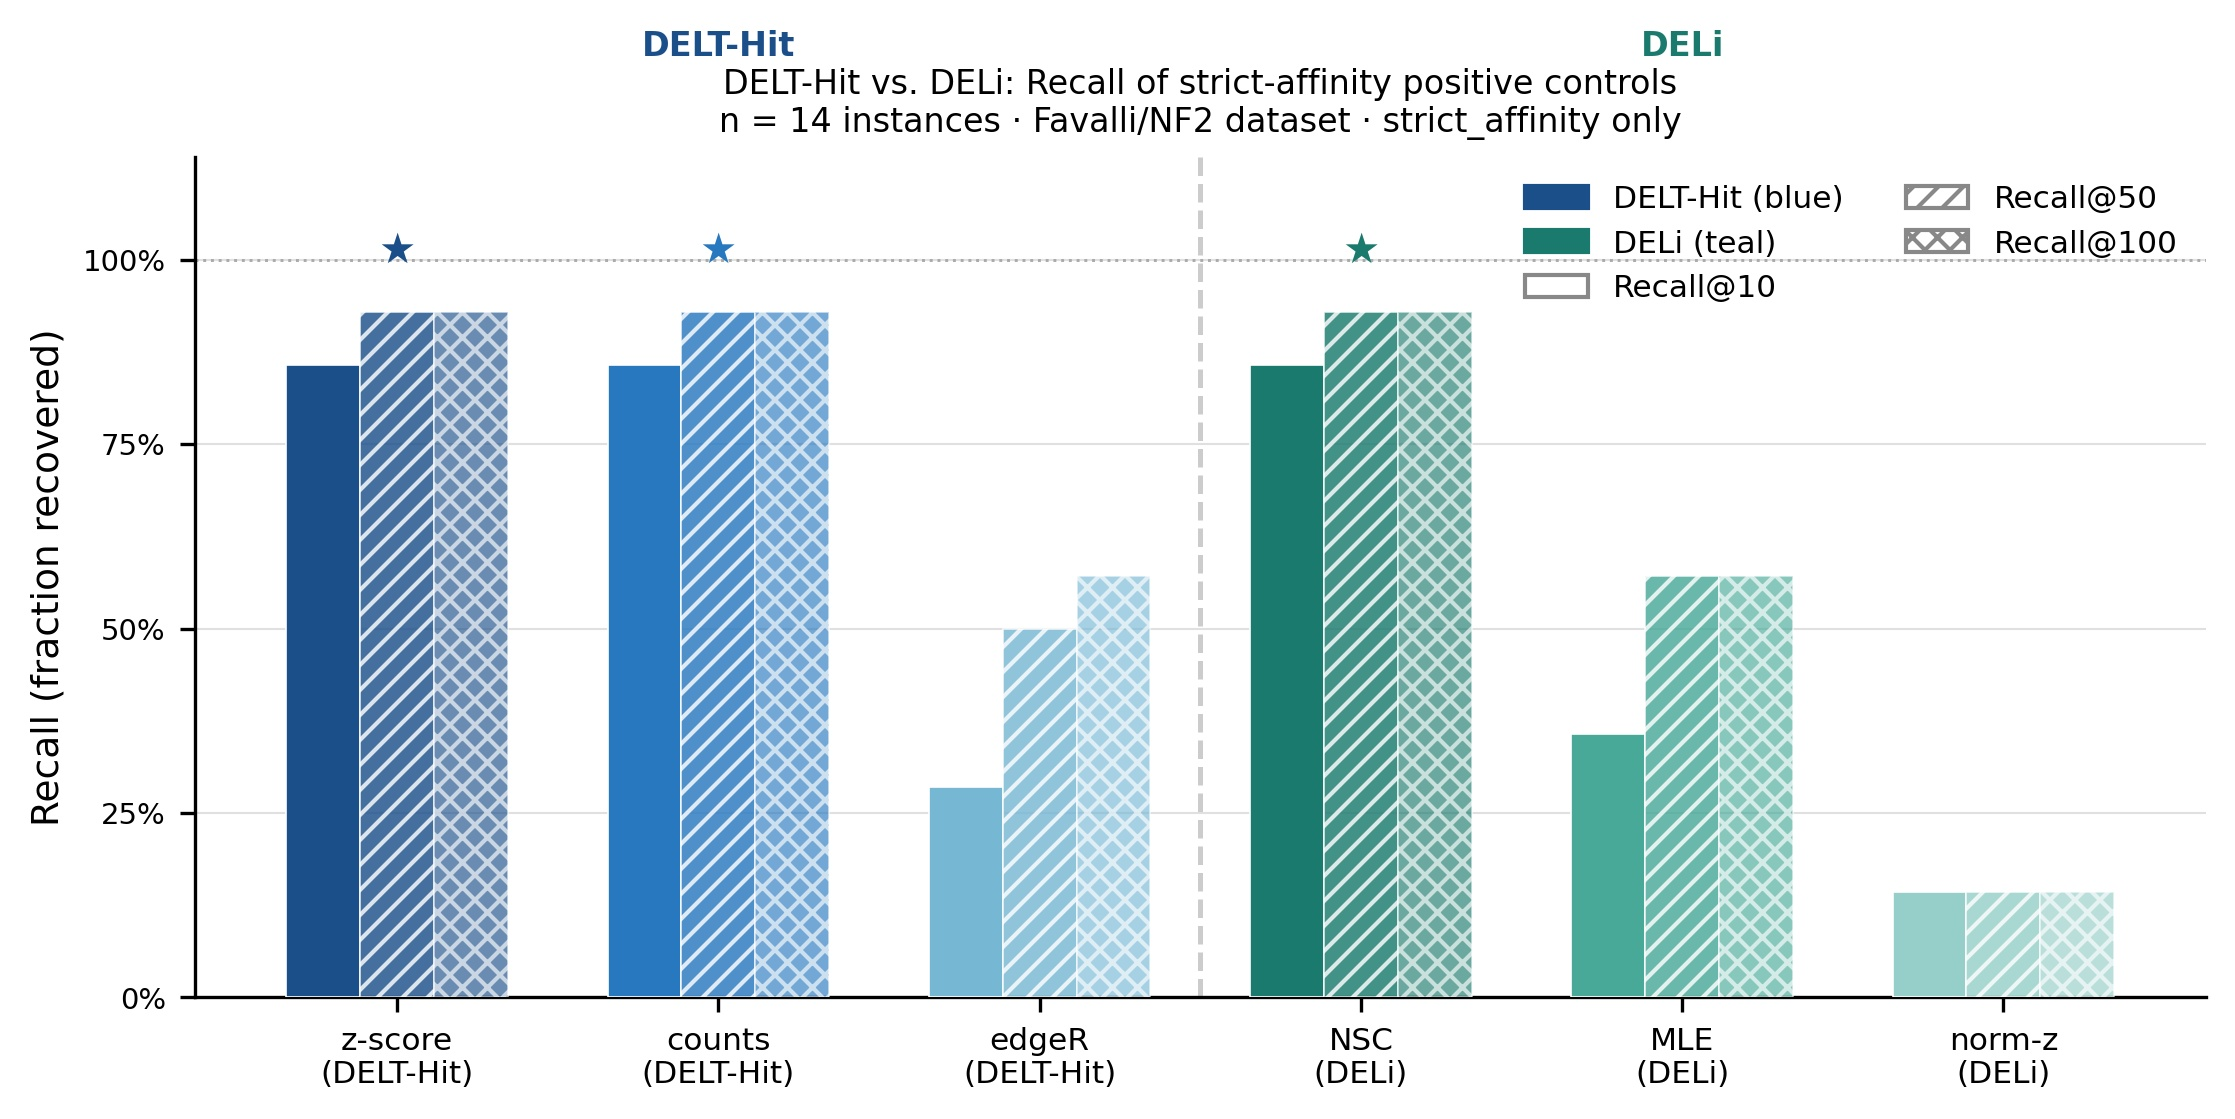
\includegraphics[width=0.85\linewidth]{figures/nf2_strict14_delt_vs_deli_recall_palette1.jpg}
\caption{\textbf{\delthit{} vs.\ \deli{} Recall at fixed rank cutoffs ($n = 14$).}
Recall@10 (solid), Recall@50 (hatched), and Recall@100 (cross-hatched) are
shown for each method grouped by tool family. Stars ($\bigstar$) mark methods
achieving $\geq$92.9\% Recall@50.}
\label{fig:delt_vs_deli_recall}
\end{figure}

\textbf{Per-instance ranks.}
Per-instance inspection showed that 13 of the 14 strict-affinity instances were
recovered within the top 50 by the frequency-based methods. The only common miss
was H1047R-PI3K ds A110/B157, where the protein and no-protein replicates carry
nearly identical low read counts (mean 5.7 protein reads per replicate against
mean 4.3 no-protein reads, giving a protein-minus-control delta of only $\sim$1.3
reads). The compound therefore falls below the practical detection limit for
this display context. The same compound--target pair ranks near the top in the
ss condition and was validated by ELISA in the original study, so the ds result
is best interpreted as a low-count, display-context-specific miss rather than
evidence against the curated affinity assignment. The full per-instance rank
table is provided in
\path{supporting_material/experiments/favalli/benchmark_nf2/strict14_method_ranks.csv}.

\textbf{Interpretation.}
The Favalli hit table reports enrichment factors based on post-selection counts
relative to the average count in each selection. This benchmark therefore tests
whether the methods recover the published frequency-enrichment signal for
affinity-measured positives. In this setting, frequency-based ranking gives the
most reliable primary hit-recovery signal: \delthit{} counts, \delthit{}
z-score, and \deli{} NSC recover 13 of 14 strict positives within the top 50.
edgeR remains useful for significance annotation, but its logFC ranking is less
effective as the only full-library ordering criterion. The poor \deli{} norm-z
result reflects the sparse no-protein-control setting, where many compounds
have zero or near-zero control counts, and should not be read as a general
failure of \deli{}.
